\section{Exception 异常}

Java 的异常继承结构如下:

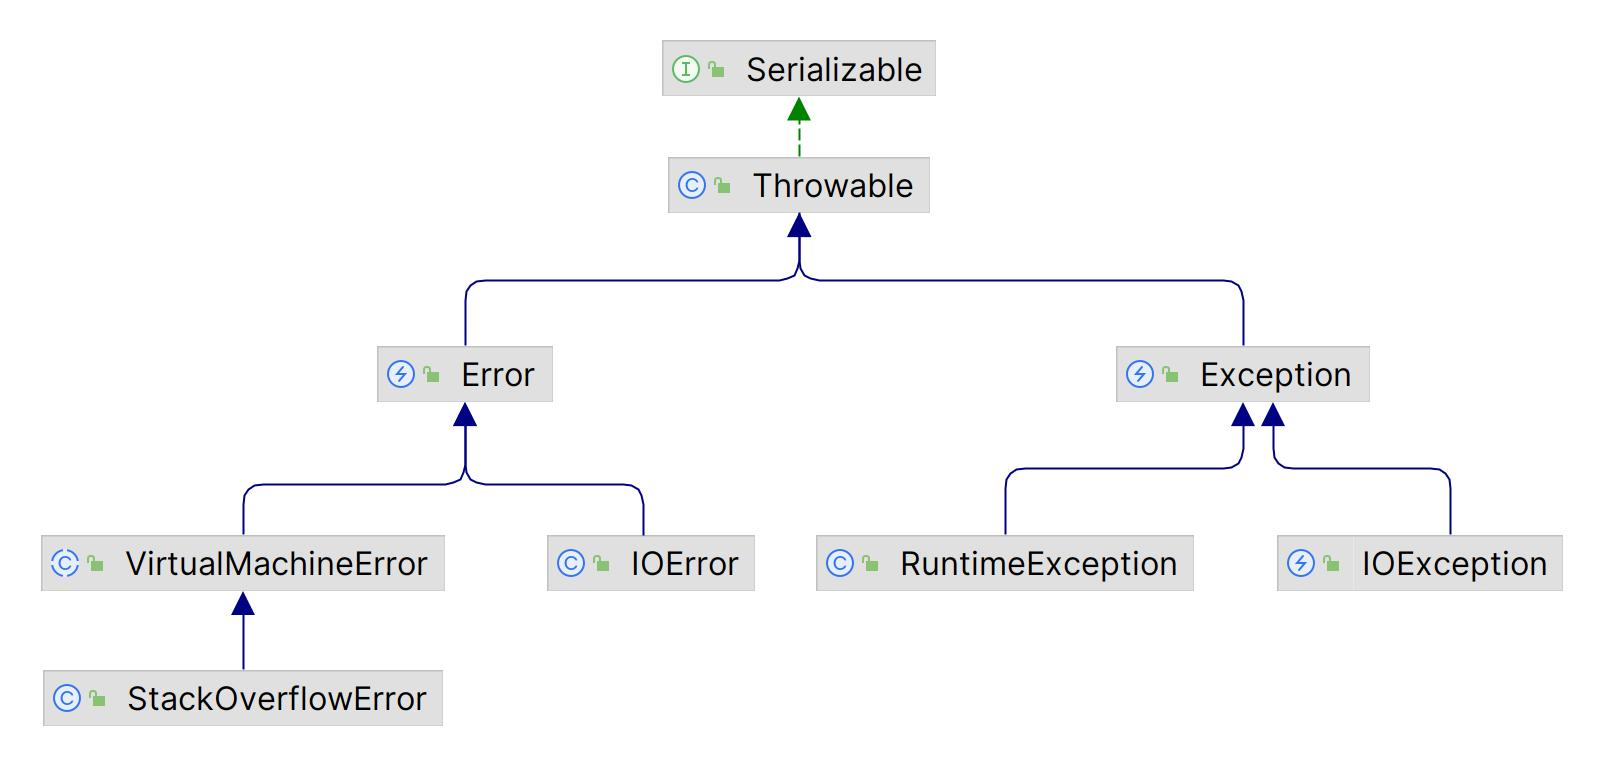
\includegraphics[width=0.9\linewidth]{../../imgs/Throwable.jpg}

Java 异常可以分为两类:检查型异常与非检查型异常:
\begin{itemize}
    \item \textbf{检查型异常}
    \begin{itemize}
        \item 范围:Error 与 RuntimeException 以外的异常
        \item 定义:编译器要求必须处理的异常,编译器会在编译前检查代码,没处理这些异常不能编译。
        \item 处理:继续 throws 抛出,或者 try...catch 处理。
    \end{itemize}
    \item \textbf{非检查型异常}
    \begin{itemize}
        \item 范围:Error 与 RuntimeException
        \item 定义:编译器不要求强制处置的异常,虽然你有可能出现错误,但是我不会在编译的时候检查,没必要,也不可能。
        \item 处理:捕获,抛出需要程序员预知有这些错误,不会静态提示。或者不处理,让程序出错。
    \end{itemize}
\end{itemize}

也可以分为运行时异常与非运行时异常:

\begin{itemize}
    \item 运行时异常:RunTimeException 都是非检查型异常,例如空指针,下标越界,一般是逻辑错误引起的。
    \item 非运行时异常:RunTimeException 以外的异常,从语法角度将必须在编译前处理。
\end{itemize}

\subsection{Error}

Error 的源码非常简单,抛出错误时可以携带消息或者错误原因,其他错误的源码也几乎一样,部分源代码如下:

\begin{Java}
public class Error extends Throwable {
    public Error(String message) {
        super(message);
    }
    public Error(String message, Throwable cause) {
        super(message, cause);
    }
    public Error(Throwable cause) {
        super(cause);
    }
}
\end{Java}

\newpage